\normallinespacing

\chapter{Introduction}

\section{Context}

The online education field has been growing continuously in the last decade, and it became essential in several countries due to COVID-19 pandemic\footnote{http://www.guide2research.com/research/online-education-statistics}. Online courses use assignments and quizzes to offer interactive learning environments to students. Massive open online courses (MOOC) are able to reach a large number of students due to their automatic assessment systems. In fields related to mathematics or computer programming, assessments can be easily automated. In music performance education, automatic assessment is much more difficult. Apart from the subjectivity of the task \cite{wesolowski2016examining}, audio recordings from students must be analysed correctly to make an accurate assessment and provide meaningful feedback. Music Information Retrieval (MIR) field focuses on tasks (onset detection, chord detection, score alignment and many more) that can make such analysis possible. 

MusicCritic \cite{bozkurt2018musiccritic} is a software framework developed to provide external automatic music performance assessment to online education platforms. It is being used in a MOOC for North Indian classical music provided by online education platform Kadenze\footnote{https://www.kadenze.com/programs/north-indian-classical-music}. It is also tested on the MOOC "Guitar for Beginners" by Berklee College of Music\footnote{https://www.kadenze.com/courses/guitar-for-beginners/}.  

\begin{figure}
    \centering
    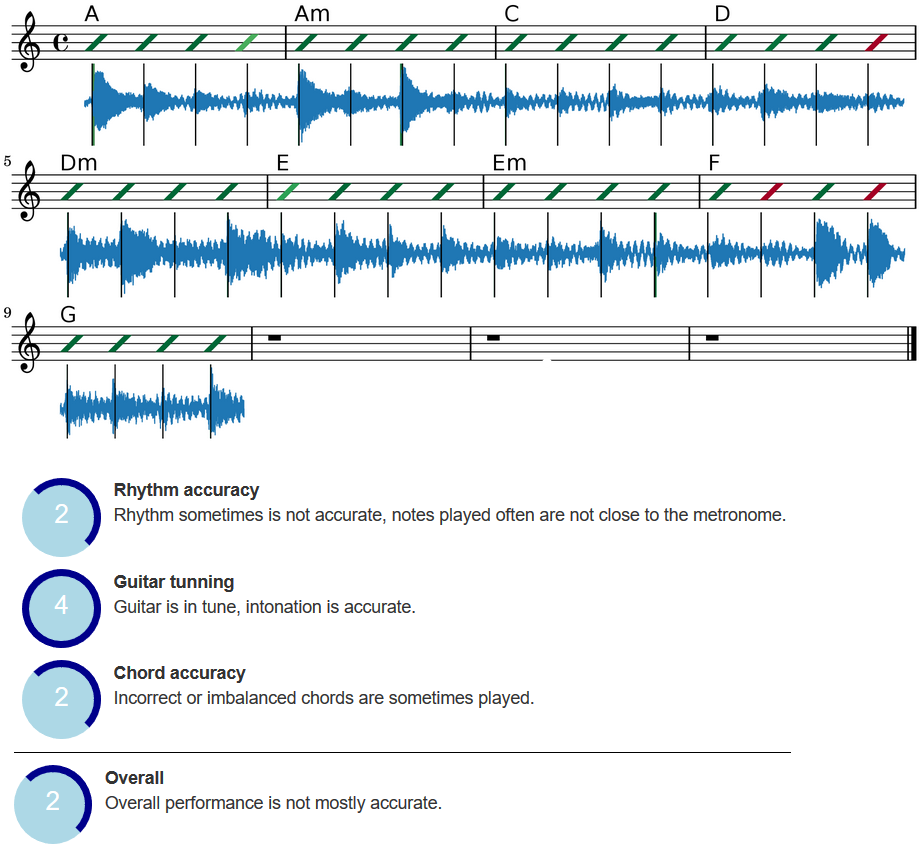
\includegraphics[width=\columnwidth]{introduction/mciritic.png}
    \caption{MusicCritic's feedback interface for a strumming exercise}
    \label{fig:musiccritic}
\end{figure}

\section{Motivation and Objectives}

In automatic assessment systems, the correctness and quality of the played notes and chords are determined by analysing their audio segments and comparing harmonic features with expected results. Accuracy of the assessment in any criteria, particularly rhythm, strictly depends on correct detection of locations of played notes. Therefore onset detection is arguably the most important part of an automatic assessment system.

Guitar players need to move their hands and interact with strings quickly and accurately. Due to its nature of the instrument, unintended noises occur often. Some of these noises (e.g. slide noise) even became a characteristic of guitar and generated by synthesizers to make the audio more realistic. Those noises do not add any musical meaning to the performance. Beginner players, who do not have hand coordination skills yet, generate plenty of noises. For instance, pressing the strings with incorrect posture or weak force usually causes a "buzz" noise, as a result of a loose string collapsing frequently with a fret. Noise events, just like the played notes, change the spectral content in the recorded signal. An onset detection algorithm for a MOOC on guitars must be robust against such noises for the aforementioned reasons. 

In many MIR tasks, most algorithms are developed and tested on high-quality recordings; the players are skilled and recording environments are adequate. Also, there is a post-processing step if it is a commercial recording. Those algorithms show inferior performance on amateur recordings. Most onset detection algorithms in literature also do not address amateur recordings. They are not very useful for applications where users are not highly skilled and the recording environment is non-ideal (e.g. noisy, reverberant), especially if the instrument is a guitar and the player is a beginner. 

Music teachers can distinguish the noises from intended notes easily and assess the performance accordingly. An assessment system to be used in a MOOC for guitars must have a very accurate onset detection algorithm. This is necessary for fair grading, and especially for correct feedback to the students. A grading system, possibly a machine learning algorithm, could tolerate a few detection mistakes. But on a feedback given to the students, obvious mistakes would harm the reputation of the assessment system and the online course.

Objectives of this work are

\begin{itemize}
  \item Evaluate several onset detection algorithms on guitar recordings, including the state of the art algorithm and the one currently being used in MusicCritic.
  \item Develop a better onset detection algorithm by considering the complications of amateur recordings.
  \item Improve the automatic rhythm assessment results using the new onset detection algorithm.
\end{itemize}

We use the rhythm assessment to measure the effect of onset detection algorithms on the overall system since the rhythm assessment depends only on (perceived) onset locations. 

\section{Thesis Organization}

In the next chapter, onset detection methods are reviewed and some studies on perceived attack time are discussed. In chapter 3, the datasets used in this study are described. In chapter 4, annotations of the datasets and evaluations of onset detection and automatic rhythm assessment experiments are explained.

In chapter 5, characteristics of the common noises in guitar recordings are examined. Insights gained from this chapter are used in the development of the new onset detection algorithm, which is explained in chapter 6. Onset detection and automatic rhythm assessment results are presented in chapter 7, followed by discussion and conclusion chapters.

\newpage


